\chapter{The beyond Standard Model of particle physics}\label{chp:BSM}
This Chapter describes the motivations for new theories beyond the Standard Model (BSM) in Section \ref{sec:BSM} and introduces some BSM theories that predict the existence of heavy resonances which can decay to a dilepton final state \footnote{In this thesis, the expression ``dilepton final state''  denotes the decay in electron-positron pair ($\mathrm{e^{+}e^{-}}$) or muon-antimuon pair ($\mu^{+}\mu^{-}$).} in Section \ref{sec:HeavyResonance}. Finally, an introduction to the search for new physics in top quark production is given in Section \ref{tW_Int}.

\section{Motivation for new physics} \label{sec:BSM}
Despite the tremendous success of SM, there are still some shortcomings about it. Such as the existence of neutrino mass \cite{Fukuda:1998mi,Abe:2011fz}, the existence of dark matter and dark energy \cite{Rubin:1970zza,Freese:2008cz} and the matter-antimatter asymmetry. All of these observations can not be explained by SM. Besides, there are some limitations for the SM, such as lack of gravity description, convergence of the coupling constants \cite{const_running}. Finally, the hierarchy problem and the existence of large number of free parameters in SM \cite{Olive:2016xmw} make it looks unnatural. Therefore, it is commonly admitted that the SM is an effective model of a more fundamental theory at high energy. Each of these issues is shortly described in below.

%\begin{itemize}
\begin{enumerate}

\item[$\bullet$]\textbf{Neutrino mass:} In the SM, the neutrino is assumed to be massless. However, it is observed that neutrinos can change from one flavour to another flavour which implies that they must have non-zero mass differences \cite{Fukuda:1998mi,Abe:2011fz} and their mass eigenstates are different from their flavour eigenstates. Experimentally, only upper limits on the neutrino masses have been set ($m<2$ eV \cite{Olive:2016xmw}). In addition, the differences between the neutrino squared masses have been measured: $\Delta m_{12}^{2}=(7.53\pm 0.18)\times10^{-5}~\mathrm{eV^{2}}$ and $\Delta m_{32}^{2}=(2.44\pm 0.06)\times10^{-3}~ \mathrm{eV^{2}}$ \cite{1674-1137-38-9-090001}.


\item[$\bullet$]\textbf{Dark matter and dark energy:} Some astronomical observations show that the visible content of matter is only be $\sim5\%$ of the total matter and energy content of the universe. Firstly, it is measured that the orbital velocities of stars around their galaxy center are too fast \cite{Rubin:1970zza,Freese:2008cz} which is incompatible with the observed matter density in space.
    In order to solve the conflict between the experimental result and the theory prediction, the existence of ``dark'' matter which does not interact via electromagnetic or strong interaction has been proposed.
    Secondly, it is discovered that the universe is in accelerated expansion which means the galaxies are recede from each other and their escape rate increases with the distance \cite{Riess:1998cb,Perlmutter:1998np}. Giving these two cosmological results, one can conclude that the matter (or energy) content of the universe is made of $5\%$ ordinary matter, $25\%$ dark matter and $70\%$ dark energy which gives repellent force and is thought to be responsible for the observed accelerated expansion of the universe. However, the SM does not provides the candidates for dark matter as well as it can not explain the dark energy problem.

\item[$\bullet$]\textbf{Asymmetry between matter and antimatter:} It is believed that matter and antimatter were produced with the same quantities at the time of Big Bang. However, we are living in a world composed with matter. So why does this happen and is it possible that some corners of the universe are dominated by antimatter$?$ In 1967, Sakharov identified the three mechanisms necessary to obtain a global matter or antimatter asymmetry \cite{SAKHAROV}:
     \begin{itemize}
     \item Baryon and lepton number violation;
     \item Interactions in the universe out of thermal equilibrium at a given moment of the universe history;
     \item Charge (C) and charge-parity (CP) violation (the rate of a process $i\rightarrow f$ can be different from the CP conjugate process $\bar{i}\rightarrow\bar{f}$).
     \end{itemize}
    The SM includes sources of CP violation: one is from a complex phase factor in the Cabibbo-Kobayashi-Maskawa (CKM) \cite{PhysRevLett.10.531,10.1143/PTP.49.652} unitary matrix (which contains information on the strength of the flavour-changing weak interaction), and the other in the form of the QCD vacuum angle, $\theta_{\mathrm{QCD}}$ \cite{RevModPhys.70.323}. However, they are not sufficient to explain the magnitude of the observed matter-antimatter asymmetry.

\item[$\bullet$]\textbf{Free parameters of the SM:} There are 19 free parameters which have to be measured in the SM. The parameters include the masses of charged lepton, the masses of quark, the coupling constants of the three forces, the mass and vacuum expectation value of the Higgs boson, the mixing angles and the CP violating phase of the CKM matrix \footnote{In addition, there are 7 parameters come from neutrino section: 3 neutrino masses, 3 mixing angles between different neutrinos, and 1 CP violating phase.}. Due to this large number of free parameters, it is widely believed that there could be a more general and elegant theory than the SM. The list of parameters is summarized in Table \ref{SM_parameters}.

\begin{table}[!htb]
  \begin{center}
    \begin{tabular}{ccc}
      \hline
      Quantity & Symbol & Value\\ \hline
Electron mass & $m_\mathrm{e}$ & 511 keV\\
Muon mass     & $m_\mathrm{\mu}$ & 105.7 MeV\\
Tau mass      & $m_\mathrm{\tau}$ & 1.78 GeV\\
Up quak mass  & $m_\mathrm{u}$    & 2.3 MeV ($\mu_\mathrm{\overline{MS}}$=2 GeV)\\
Down quak mass  & $m_\mathrm{d}$    & 4.8 MeV ($\mu_\mathrm{\overline{MS}}$=2 GeV)\\
Strange quak mass  & $m_\mathrm{s}$    & 95 MeV ($\mu_\mathrm{\overline{MS}}$=2 GeV)\\
Charm quak mass  & $m_\mathrm{c}$    & 1.28 GeV ($\mu_\mathrm{\overline{MS}}=m_\mathrm{s}$)\\
Bottom quak mass  & $m_\mathrm{b}$    & 4.18 GeV ($\mu_\mathrm{\overline{MS}}=m_\mathrm{b}$)\\
Top quak mass  & $m_\mathrm{t}$    & 173.5 GeV\\
W boson mass & $m_\mathrm{W}$ & 80.4 GeV\\
Z boson mass & $m_\mathrm{Z}$ & 91.2 GeV\\
Higgs boson mass & $m_\mathrm{H}$ & 125.09 GeV \cite{higgs_mass}\\
Higgs boson vacuum expectation value & $v$ & 246 GeV\\
Strong coupling constant & $\alpha_s$ & 0.119 ($\mu_\mathrm{\overline{MS}}=m_\mathrm{Z}$)\\
QCD vacuum angle & $\theta_\mathrm{QCD}$ & $\sim 0$\\
CKM 12-mixing angle & $\theta_\mathrm{12}$ & 12.9\textdegree\\
CKM 23-mixing angle & $\theta_\mathrm{23}$ & 2.4\textdegree\\
CKM 13-mixing angle & $\theta_\mathrm{13}$ & 0.2\textdegree\\
CKM CP violating phase & $\delta_\mathrm{13}$ & 69\textdegree\\
      \hline
    \end{tabular}
\caption{The SM parameters. The quark masses are presented in the renormalization scheme known as $\mathrm{\overline{MS}}$ \cite{Olive:2016xmw}.}
\label{SM_parameters}
  \end{center}
\end{table}

\item[$\bullet$]\textbf{Gravitational interaction and hierarchy problem:} The gravity, the fourth fundamental interaction, is not included in the SM because of its very small interaction strength compared with other three forces. The electromagnetic, weak and strong forces have similar strengths at the electroweak scale (energies of $\approx$ 100 GeV), but gravity is more than $10^{30}$ times weaker. The energy at which gravitational interactions becomes relevant is at the order of the Planck scale of $E_{Pl} = 10^{19}$ GeV, which is defined by the Planck mass, $M_{Pl} =\sqrt{\hbar c/G}$, where $G$ is the gravitational constant. The huge difference between the electroweak scale and the Planck scale is also known as the hierarchy problem and it is deeply connected to the problem of the Higgs boson mass fine-tuning (which is expressed in the following).
    %Gravity is very different from the three other forces in many aspects and establishing a common framework to describe both faces several difficulties.
%    General relativity (GR) indicates that gravity is deeply connected to the space-time geometry and that it couples to the particles energy-momentum tensor, which makes its integration to the SM more subtle than simply adding a new interaction. Besides, in order to combine the quantum theory of the SM with the GR,
%    a quantum theory of gravity is necessary and this would lead to a new field associated to gravity which is a spin 2 particle, called graviton. Moreover,


\item[$\bullet$]\textbf{Fine-tuning of the Higgs boson mass:} All the ingredients of the SM have been experimentally established after the discovery of the Higgs boson and the measurement of its mass ($\approx$ 125 GeV). All particles in the SM have a \textit{bare mass} which is the mass obtained from the quantum propagator at the lowest order in perturbation theory. This is can be different from \textit{physical mass} which contains higher order loop radiative corrections and can be measured in experiment.

    It is known \cite{Martin:1997ns} that the squared Higgs physical mass ($m_\mathrm{H}$) can be obtained by the squared bare mass ($m_0$) of Higgs corrected with an extra term which includes higher order corrections ($\delta m^2_\mathrm{H}$):
\begin{equation}
m^2_\mathrm{H} = m^2_0 - \delta m^2_\mathrm{H}
\label{higgs_mass}
\end{equation}
where $\delta m^2_\mathrm{H}$ includes all contributions from radiative corrections to the Higgs propagator.
The main contributions include the top quarks, the Higgs boson itself, and the vector bosons.
The related Feynman diagrams are shown in Figure \ref{ren_higgs}, where the Higgs boson is denoted as $h$ \cite{Olive:2016xmw}.

\begin{figure}[!htbp]
\begin{center}
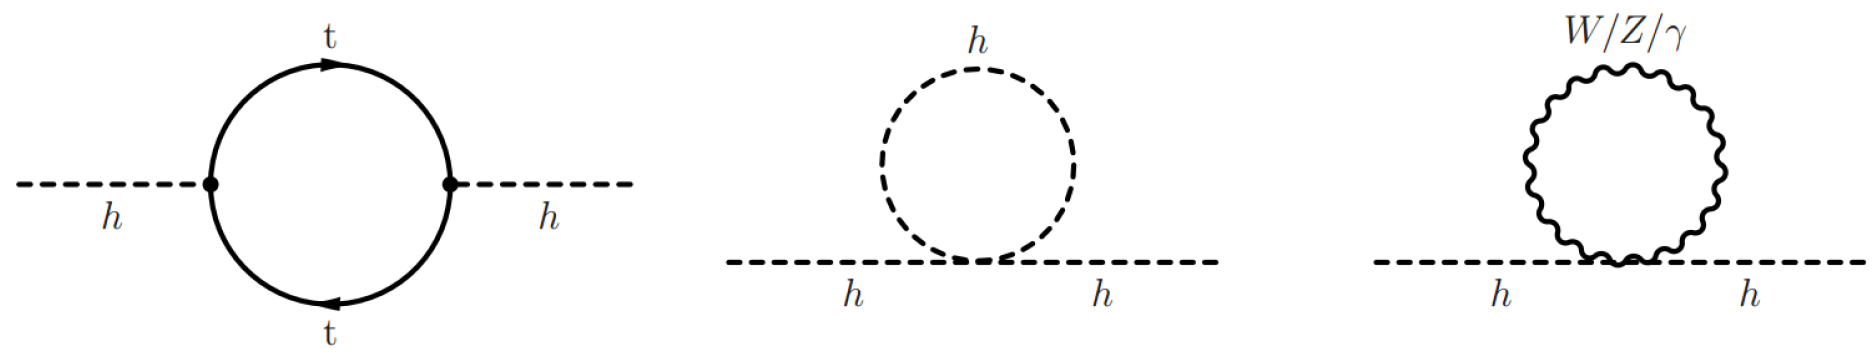
\includegraphics[width=0.9\textwidth]{figures/theory/higgs_loop.png}%scale=1.5
\caption{The Feynman diagrams of the processes which give the main divergent contributions to the Higgs boson mass.}
\end{center}
\label{ren_higgs}
\end{figure}


However, the integrals corresponding to the amplitude of these processes are divergent, so a cut-off parameter $\Lambda$ is introduced. The $\Lambda$ represents the energy scale, up to which the SM is still valid. In principle, one can assume that the SM is valid up to the Planck scale at which gravitational effects cannot be neglected. With this assumption $\Lambda$ would be of the order of $\approx 10^{19}$ GeV. The full calculation gives that $\delta m^2_\mathrm{H}$ is proportional to $\Lambda^2$:
\begin{equation}
\delta m^2_\mathrm{H} \propto \Lambda^2 \approx 10^{38}~\mathrm{GeV^2}
\end{equation}
Because $m_\mathrm{H}$ is $\approx 125$ ($\approx 10^2$) GeV, Equation (\ref{higgs_mass}) can be rewritten as:
$$10^4~\mathrm{GeV^2} \approx  m^{2}_0 -\Lambda^2 \approx m^2_0 -10^{38}~\mathrm{GeV^2}$$
which means that $m^2_0$ is of the same order of $\Lambda^2$ ($10^{38}$) and these two terms
cancel with a very high precision to obtain the value of the Higgs physical mass. This
mathematical problem is called ``Higgs mass fine-tuning'' problem, although it does not invalidate the theory. However, it seems an unnatural and implausible coincidence that $m^2_0$ cancels all the loop contributions up to this astonishing precision.

Actually, the problem comes from the choice of the $\Lambda$. If we choose the $\Lambda$ to be $\approx$ 1 TeV, then the problem is solved because the cancellation is of the order of one over ten which seems is a natural and acceptable value.
For this reason, if one accepts the Higgs mass fine-tuning argument, then the new physics will appear at the TeV scale, because at energy higher than $\Lambda=$ 1 TeV, the SM is not valid anymore.


%The choice of $\Lambda$ made in the previous calculation is somehow arbitrary because it
%is based on the assumption that the SM is still valid up to the greatest
%possible energy, the Planck scale. If a lower $\Lambda$ is chosen, the cancellation is tuned to
%an acceptable level. For instance, $\Lambda\approx$1 TeV is chosen, the hierarchy problem is
%completely solved since the cancellation is of the order of one over ten, which seems
%a natural and acceptable value.


\item[$\bullet$]\textbf{Convergence of the coupling constants}: In SM, the coupling strengths for electromagnetic interaction, weak interaction, and strong interaction have a close value at the energy scale $\mathcal{O}(10^{16})$~GeV. However, these three coupling strengths can not converge at a single point which is shown in Figure~\ref{fig:couplings}. In order to unify these couplings, an extension of the SM is needed and the new physics will be involved.
%The SM coupling constants of the strong interaction, the electromagnetic interaction and the weak interaction have a similar value at an energy scale of $\mathcal{O}(10^{16}$~GeV). However, they do not converge to a single value as shown in Figure~\ref{fig:couplings}. In order to unify the coupling constants, an extension of the SM would be necessary in order to modify their evolution above the electroweak scale.

\begin{figure}[!htbp]
	\begin{center}
		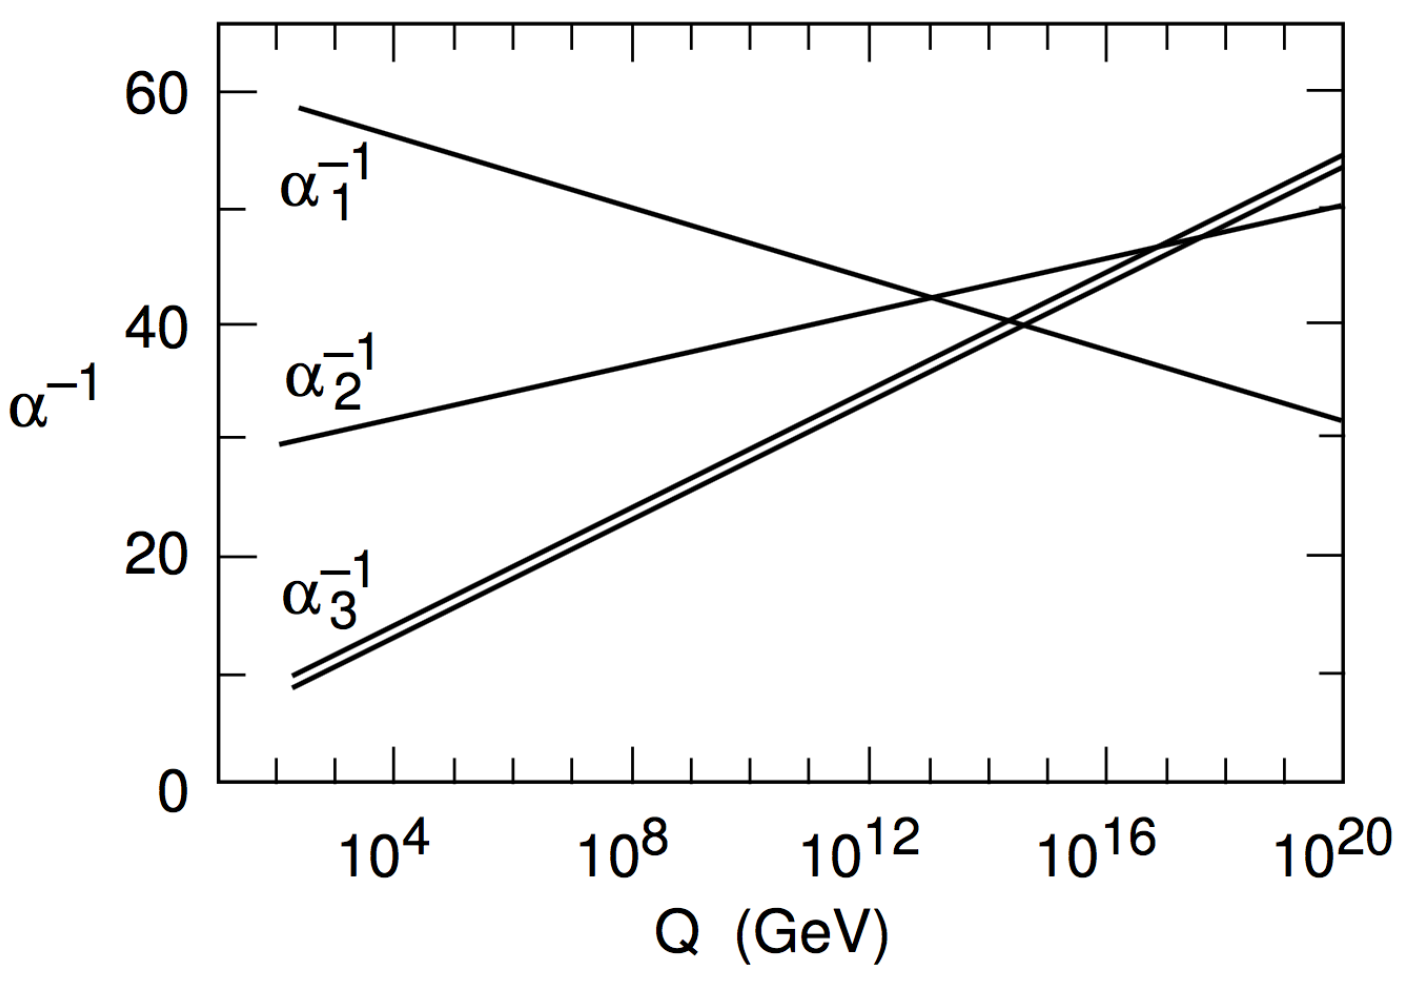
\includegraphics[width=0.7\textwidth]{figures/theory/SMcouplings.png}
	\end{center}
	\caption{Evolution of the SM couplings
	$\alpha_i = \frac{g_i^2}{4\pi}$ as a function of the energy scale~\cite{const_running}.
	}
\label{fig:couplings}
\end{figure}
%\end{itemize}
\end{enumerate}
All these issues indicate that there must be new physics at a scale beyond the electroweak scale. Driven by the hierarchy problem, it is believed that there should be new physics at the TeV scale. Therefore, a discovery with direct searches at the Large Hadron Collider (LHC) could be possible.


\section{New heavy particles decaying into a lepton pair}\label{sec:HeavyResonance}
The most directly way to search for a new heavy particle decaying into a lepton pair would be searching for the ``bump'' (or localized excess) in dilepton mass spectrum at high mass. This study is motivated both theoretically and experimentally. From a theoretical point of view, many beyond SM (BSM) models predict the existence of new massive resonances which can decay into dilepton. Such as:
\begin{enumerate}
\item[$\bullet$] The supersymmetric model \cite{Barbier} which is extremely attractive, because it can provide an explanation to the Higgs mass fine-tuning problem. In order to avoid issue of naturalness for the Higgs boson mass, the supersymmetric particles cannot be
much heavier than 1 TeV which makes searching for these new particles is doable at LHC. Besides, the supersymmetric models provide a natural candidate of dark matter. There are many supersymmetric models, the simplest one is the Minimal Supersymmetric Standard Model (MSSM) where each SM particle has a superymmetric partner. The fermions have spin 0 ``sfermion'' partners, gauge bosons have spin $\frac{1}{2}$ ``gaugino'' partners and the super-partner for higgs is ``higgsinos''.
In SM, the baryon (B) number and lepton (L) number are conserved, where $\mathrm{B=\frac{1}{3}(n_q-n_{\overline{q}})}$ and $\mathrm{L=(n_l-n_{\overline{l}})}$. However, in the MSSM the B and L can be violated. In order to maintain the experimentally verified conservation laws, one defines a new conserved quantum number, the R-parity $\mathrm{P_R}$ as:
$$\mathrm{P_R=(-1)^{3B-L+2s}},$$
where s is the spin of the particle. For the SM particles the $\mathrm{P_R}=+1$ and for supersymmetric particles the $\mathrm{P_R}=-1$. Due to the conserved $\mathrm{P_R}$, the supersymmetric particles can not decay into dilepton final states. However, in more complicated supersymmetric model \cite{BARBIER20051} where the $\mathrm{P_R}$ can be violated, the new particles (e.g. ``sneutrinos'') can decay into dilepton final states.


\item[$\bullet$] The Grand Unified Theory (GUT) \cite{Altar:1989,Leike,Rizzo} which tries to unify electromagnetic, weak, and strong interactions into one interaction through the extensions of the SM gauge group is also attractive. There are many GUT models, the starting point is the $SU(5)$ \cite{Glashow} model which was initially proposed by Georgi and Glashow in 1974. $SU(5)$ is the smallest gauge group that can contain the SM (can be expressed by $SU(5)\supset SU(3)_c \times SU(2)_L \times U(1)_Y$). It supposes the coupling strengths of electromagnetic ($g_1$), weak ($g_2$), and strong ($g_3$) interactions will merge into a single coupling ($g_G$) at the energy scale $\mathcal{O}(10^{16})$ GeV (which is called the unification scale). Besides, it predicts the $\mathrm{sin^2\theta_W}$ = 0.375 at the unification scale, and this was compatible with the measurements at that time. However, the $\mathrm{sin^2\theta_W}$ = 0.375 is now ruled out by most precise measurements and consequently $g_1$, $g_2$ and $g_3$ do not converge at single point. Moreover, in $SU(5)$ the decay of proton is allowed (e.g. $p\rightarrow e^{+}+\pi^0$), while the predicted half time of the proton decay is several orders of magnitude smaller than the experimental lower limits. Therefore, it seems the simplest $SU(5)$ is not a correct GUT model.

    Another famous GUT model is $SO(10)$ \cite{King:1981ge} which was proposed by H. Fritzsch and P. Minkowski in 1975. In $SO(10)$ all matter particles belonging to the same generation are grouped into a single multiplet and has the nice feature to predict an half time for the proton decay which is not in contradiction with the experimental results. In $SO(10)$, the symmetries can be broken at different scale. For instance, the breaking scheme for $SO(10)$ could be:
    $$SO(10)\rightarrow SU(5)\times U(1)_\upchi\rightarrow G_{SM}\times U(1)_\upchi$$
    where $G_{SM}$ is $SU(3)_c \times SU(2)_L \times U(1)_Y$ and $\upchi$ is the charge associated to the extra $U(1)_\upchi$ group. There is no constraint on the breaking scale for this $U(1)_\upchi$ and it might happen at the TeV scale.


Moreover, the $E_{6}$ model \cite{Witten:1985xc} is also popular which is able to embed $SU(5)$ lie on the exceptional $E_{6}$ group. The $E_{6}$ group can break down to SM by following scheme:
$$E_6\rightarrow SO(10) \times U(1)_\uppsi \rightarrow SU(5)\times U(1)_\upchi \times U(1)_\uppsi\rightarrow G_{SM}\times U(1)_\upchi \times U(1)_\uppsi.$$
The new particle \ZP from the linear combination of $U(1)_\upchi$ and $U(1)_\uppsi$ is given by:
$$\ZP=\mathrm{\ZPPSI cos\theta_{E_6} + \ZPCHI sin\theta_{E_6}}$$
where  $\mathrm{0\leq\theta_{E_6}\leq\pi}$ is a mixing angle. Therefore, different $\mathrm{\theta_{E_6}}$ will give different \ZP.


Some specific $\mathrm{Z^{'}s}$ are: 1, the \ZPPSI ($\mathrm{\theta_{E_6}}=0$) that only interacts through axial-vector couplings with the fermions and it is predicted by superstring theories \cite{WITTEN198575}. 2, the \ZPCHI ($\mathrm{\theta_{E_6}}=-\frac{\pi}{2}$) that corresponds to a pure $U(1)_\upchi$ group. 3, the \ZPETA ($\mathrm{\theta_{E_6}=arccos}\sqrt{\frac{5}{8}}$), also suggested by superstring theories \cite{WITTEN198575}. 4, the \ZPI ($\mathrm{\theta_{E_6}}$=(arccos$\sqrt{\frac{5}{8}}$)-$\frac{\pi}{2}$) that does not couple to up quarks and only couples to left-handed down quarks and right-handed leptons. The couplings between these specific $\mathrm{Z^{'}s}$ and the up quarks, the down quarks, and the charged leptons can be seen in Table \ref{zprime_couplings}.

Last but not least, the Sequential Standard Model (SSM)~\cite{Altar:1989} \ZP has couplings which are exactly the same as those of the SM Z (see Table \ref{zprime_couplings}), but is just heavier. This is not a real model but is very commonly used as a ``standard candle'' in experimental \ZP (or $\mathrm{W^{'}}$) searches.


\begin{table}[!htb]
\begin{center}
\begin{tabular}{|c||c|c|c|c|c|c|c|}
      \hline
      Model          & $\mathrm{\theta_{E_6}}$                       & $c^{u}_{V}$ & $c^{u}_{A}$ & $c^{d}_{V}$ & $c^{d}_{A}$ & $c^{l}_{V}$ & $c^{l}_{A}$ \\ \hline
      \ZPPSI         &  0                                            & 0           & 0.301    & 0           & 0.301    & 0           & 0.301    \\
      \ZPETA         &  arccos$\sqrt{\frac{5}{8}}$                   & 0           & 0.380    & -0.285   & 0.0950    & 0.285    & 0.0950    \\
      \ZPCHI         &  -$\frac{\pi}{2}$                             & 0           & 0.0735    & -0.416   & -0.343   & 0.416    & -0.343   \\
      \ZPI           &  (arccos$\sqrt{\frac{5}{8}}$)-$\frac{\pi}{2}$ & 0           & 0           & 0.621    & -0.621   & -0.621   & -0.621   \\ \hline
      \ZPSSM         &  --                                           & -0.227   & 0.593    & 0.410    & -0.593   & 0.0446    & -0.593   \\
      \hline
    \end{tabular}
\caption{The specific \ZP bosons with corresponding $\mathrm{\theta_{E_6}}$ form $\mathrm{E_6}$ model together with the vector ($c_V$) and axial ($c_A$) couplings between the \ZP and the up quarks ($u$), the down quarks ($d$), and the charged leptons ($l$). The \ZPSSM from the Sequential Standard Model which has the same SM couplings is also shown.}
\label{zprime_couplings}
\end{center}
\end{table}


\item[$\bullet$] In order to explain the large difference between the electroweak scale ($\mathcal{O}$(100) GeV) and the Planck scale ($\mathcal{O}(10^{19})$ GeV), the theories involve extra dimensions are proposed. It is assumed that there exist a spin 2 graviton (the carrier of the gravitational interaction and can decay into dielectron or dimuon pair) that can propagate in extra dimensions which have small radius $R$ ($R$ should be less than 100 $\mu$m \cite{Schwarz} and assuming all the extra dimensions share the same radius), while SM forces are confined in usual 4-dimension spacetime. Due to the overlap of the wave functions of the SM particles with the graviton is small in 4-dimension spacetime, the gravity is much weaker than other three forces in our 4-dimension world. There are many extra dimensions models, such as ADD model (proposed by Arkani-Hamed, Dimopulous and Dvali) \cite{arkani98:hlz} which is one of the first solutions of the hierarchy problem by involving extra spatial dimensions. In ADD model, the $R$ decreases with the increases of the number of extra dimension $n$. For $n=1$, the $R$ is around $10^{11}$ m at which distances the Newton's law is well established. However, the prediction from ADD for $n=1$ gives deviations to the one from Newton's law. Therefore, $n=1$ is excluded in ADD and $n$ should start from 2 which corresponds to $R=100$ $\mu$m which is just at the experimental limits \cite{Schwarz}. Another type of extra dimension model using 5-dimensional warped geometry theory has been developed by Randall and Sundrum \cite{Sundrum} called ``Randall-Sundrum model''. The Randall-Sundrum model uses ``brane''\footnote{A brane is a physical object that generalizes the notion of a point particle to higher dimensions} to describe SM particles (``Weakbrane'') and graviton (``Planckbrane''), and gravity is much weaker on the Weakbrane than on the Planckbrane.

\end{enumerate}

Generically, the spin 1 particle that can give rise to a resonance in the dilepton mass spectrum is called \ZP, while for spin 2 particle it is called ``graviton''.

From an experimental point of view, these BSM models of new physics give rise to high energy lepton pair in the final states and the SM background for such final states is relatively low at a hadron collider. Searches for heavy resonance decaying into dilepton have been performed at LHC and Tevatron. The CMS Collaboration at the LHC performed the search with proton-proton collision data collected at $\sqrt{s}=$ 7 TeV \cite{Chatrchyan:2011wq,Chatrchyan:2012it}, with data collected at 8 TeV \cite{Chatrchyan:2012oaa,Khachatryan:2014fba}, and using the combination of 2015 data collected at 13 TeV with data collected at 8 TeV \cite{Khachatryan:2016zqb}.
Recently, CMS performed this search using the data collected at 13 TeV from 2016 \cite{Sirunyan2018} and 2017 \cite{CMS-PAS-EXO-18-006}, this search will be presented in detail in Chapter \ref{chap:Zprime}. Similar to CMS, the ATLAS Collaboration also performed the search with data collected at 7 TeV \cite{Aad:2011xp,Aad:2012hf}, with data collected at 8 TeV \cite{Aad:2014cka}, and with data collected at 13 TeV \cite{Aaboud:2017buh,Aad:2019fac}. At the Tevatron, the CDF and D0 Collaborations have published results based on a $\mathrm{p-\bar{p}}$ collision sample at $\sqrt{s} =$ 1.96 TeV, corresponding to an integrated luminosity of approximately 5 \fbinv~\cite{CDF_Zp,CDF_RS,D0_RS,D0_Zp,CDF_SSM,CDF_RSele}.


%Combining this with the high accuracy of the lepton reconstruction provided by the CMS detector makes this channel experimentally well under control. Given the large amount of models, the studies presented in this thesis (the experimental setup and results are shown in Chapter \ref{chap:Zprime}) have been conceived as model independent searches for any possible signal of a new resonance which decays to two a dilepton pair with an invariant mass above 200 GeV.






\section{New physics in top quark production}\label{tW_Int}

As described in Section \ref{sec:HeavyResonance} if the new physics scale is available at hadron collider, the existence of new physics could be directly observed via the production of new particles.
Otherwise, new physics could affect SM interactions indirectly,
through modifications of SM couplings or enhancements of rare SM processes.
In the latter case, it is useful to introduce a model-independent approach to parameterize and to
constrain possible deviations from SM predictions, independently of the fundamental theory of new physics.

Due to its large mass, close to the electroweak symmetry breaking scale, the top quark is expected to play an important role in several new physics scenarios.
An effective field theory (EFT) (See Section \ref{sec:EFT}) approach is followed in this thesis to search for new physics in the top quark sector in the ee and \mumu final states (the experimental setup and results are shown in Chapter \ref{chap:tW}).
In Refs.~\cite{Zhang:2010dr,Durieux:2014xla} all dimension-six operators that contribute to the top quark pair production (\ttbar) and the single top quark production in association with a W boson (tW) are investigated. The operators and the related effective Lagrangian, which are relevant for dilepton final states, can be written as~\cite{Grzadkowski:2010es}:
\begin{eqnarray}
\label{eq1}
\mathrm{O_{\upphi q}^{(3)}} =& \mathrm{(\upphi^+\tau^ID_\mu\upphi)(\bar{q}\gamma^\mu\tau^Iq)}  ,& L_\mathit{eff}=\mathrm{\frac{C_{\upphi q}^{(3)}}{{\sqrt 2}\Lambda^2} gv^2\bar{b}\gamma^\mu P_LtW^-_\mu+h.c.,}\\
\mathrm{O_{tW}} =& \mathrm{(\bar{q}\sigma^{\mu\nu}\tau^It)\tilde{\upphi}W^I_{\mu\nu}} ,& L_\mathit{eff}=\mathrm{-2\frac{C_{tW}}{\Lambda^2}v\bar{b}\sigma^{\mu\nu}P_Rt \partial_\nu W^-_\mu+h.c.,}\\
\mathrm{O_{tG}} =& \mathrm{(\bar{q}\sigma^{\mu\nu}\lambda^A t)\tilde{\upphi}G^A_{\mu\nu}} ,& L_\mathit{eff}= \mathrm{\frac{C_{tG}}{{\sqrt 2}\Lambda^2}v\left(\bar{t}\sigma^{\mu\nu}\lambda^A t\right) G_{\mu\nu}^A +h.c.,}\\
\mathrm{O_{G}} =& \mathrm{f_{ABC}G^{A\nu}_\mu G^{B\uprho}_\nu G^{C\mu}_\uprho} ,& L_\mathit{eff}= \mathrm{\frac{C_{G}}{\Lambda^2} f_{ABC}G^{A\nu}_\mu G^{B\uprho}_\nu G^{C\mu}_\uprho + h.c.,}\\
\mathrm{O_{u(c)G}} =&  \mathrm{(\bar{q}\sigma^{\mu\nu}\lambda^A t)\tilde{\upphi}G^A_{\mu\nu}}  ,& L_\mathit{eff}= \mathrm{\frac{C_{u(c)G}}{{\sqrt 2}\Lambda^2}v\left(\bar{u} \left(\bar{c}\right)\sigma^{\mu\nu}\lambda^A t\right) G_{\mu\nu}^A+h.c.,}
\end{eqnarray}
where \Cphiq ($\phi$ is Higgs field, q is quark), \CtW, \CtG, \CG and \CucG stand for the dimensionless Wilson coefficients, also called effective couplings.
The variable $\Lambda$ represents the energy scale beyond which new physics becomes relevant. The detailed description of the operators is given in~Refs. \cite{Zhang:2010dr,Durieux:2014xla}.
The operators \Ophiq and \OtW modify the SM interaction between W boson, top quark, and b quark (Wtb).
%The operator \OtG is called chromomagnetic dipole moment operator of the top quark.
The triple gluon field strength operator \OG represents the only genuinely gluonic CP conserving term which can appear at dimension 6 within an effective strong interaction Lagrangian \cite{Cho:1994yu}.
The operators \OuG and \OcG lead to flavor changing neutral current (FCNC) interactions of top quark and contribute to the tW production. As we know the FCNC processes do not exist at tree level in the SM and are induced only at loop level. Therefore the rates of FCNC processes are highly suppressed. The observation of such processes will be very important for searching new physics.
The effect of introducing the new couplings \Cphiq, \CtW, \CtG and \CucG can be investigated in the tW production. The \CtG affects also the \ttbar production. In the case of the \CG coupling, only the \ttbar production is modified.
It should be noted that the \OtW and \OtG operators with imaginary coefficient lead to CP-violating effects.
Representative Feynman diagrams for new physics contributions in the tW and \ttbar production are shown in Figure~\ref{fig-feyn}.
In this analysis we only probe CP-even dimension six operators via top quark production.

Several searches for new physics in the top quark sector including new non-SM couplings have been performed at the Tevatron and LHC colliders.
Results can be interpreted in two ways. Most of the previous analyses followed the anomalous coupling approach in which SM interactions
are extended for possible new interactions. In this study, the EFT framework with effective couplings is used for the interpretation of the results.
Constraints obtained on anomalous couplings can be translated to effective coupling bounds~\cite{Zhang:2010dr,Abazov:2012uga}.
A variety of limits have been set on the Wtb anomalous coupling through single top quark $t$-channel production
and measurements of the W boson polarisation from top quark decay by the D0~\cite{Abazov:2012uga}, ATLAS \cite{Aaboud:2017aqp,Aaboud:2016hsq} and CMS \cite{Khachatryan:2016sib,Khachatryan:2014vma} Collaborations.
Direct limits on the top chromomagnetic dipole moment have been obtained  by the CMS Collaboration at 7 TeV using top quark pair events~\cite{CMS:2014bea}.
Searches for top quark FCNC interactions have been performed at Tevatron~\cite{Abazov:2010qk,Aaltonen:2008qr} and at LHC~\cite{Khachatryan:2016sib,Aad:2015gea}
via single top quark production and limits are set on related anomalous couplings.

\begin{figure}[t]
\centering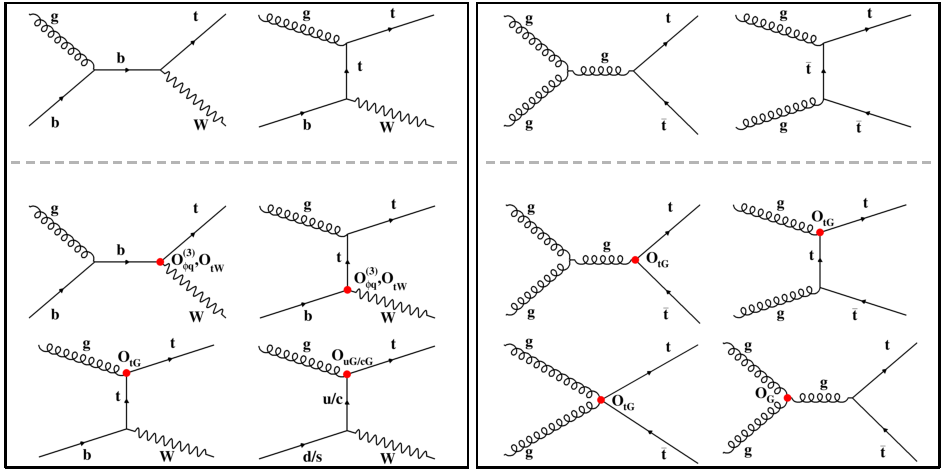
\includegraphics[width=1\textwidth]{figures/tW/fig/fey}
\caption{Representative Feynman diagrams for the tW (left panel) and \ttbar~(right panel) production at leading order. The upper row gives the SM diagrams, the middle and lower rows  present diagrams corresponding to the \Ophiq, \OtW, \OtG, \OG, and \OucG contributions.}\label{fig-feyn}
\end{figure}

\section{Summary}

In this chapter the shortcomings of SM and motivations of BSM are delivered. After that some BSM theories which predict the existence of heavy resonances decaying into dilepton are introduced. Finally, an indirect search for new physics through top production is described.

